\documentclass[11pt,a4paper]{article}
\usepackage[a4paper,margin=25mm]{geometry}
\setcounter{tocdepth}{4}
\usepackage[utf8]{inputenc}
\usepackage[T1]{fontenc}
\usepackage{lmodern}
\usepackage{amsmath}
\usepackage{amsthm}
\usepackage{amssymb}
\usepackage{mathrsfs}
\usepackage{amsfonts}
\usepackage{stmaryrd}
\usepackage{xfrac}
\usepackage{dsfont}
\usepackage{fancybox}
\usepackage{fancyref}
\usepackage{multicol}
\usepackage{graphicx}
\usepackage{wrapfig}
\usepackage{textcomp}
\usepackage{mathrsfs}
\usepackage[svgnames]{xcolor}
\usepackage{color}
\usepackage{listings}
\usepackage{tikz-cd}
\usepackage[colorlinks=true, linkcolor=black, urlcolor=blue, citecolor=black, anchorcolor=blue]{hyperref}
\usepackage{cleveref}
\usepackage{comment}
\usepackage{caption}
\usepackage{shuffle}
\usepackage{multirow}
\usepackage{appendix}
\usepackage{fdsymbol}
\usepackage{float}
\usepackage{algorithm}
\usepackage[noend]{algpseudocode}
\usepackage{qcircuit}

\newcommand{\HRule}{\rule{\linewidth}{0.5mm}}
\newcommand{\Dyck}[1]{\textsc{Dyck$_{#1}$}}
\newcommand{\FA}[1]{\textsc{FindAny$_{#1}$}}
\newcommand{\FFL}[1]{\textsc{FindFixedLength$_{#1}$}}
\newcommand{\FFP}[1]{\textsc{FindFixedPos$_{#1}$}}
\newcommand{\FALM}[1]{\textsc{FindAtLeftMost$_{#1}$}}
\newcommand{\FARM}[1]{\textsc{FindAtRightMost$_{#1}$}}
\newcommand{\FF}[1]{\textsc{FindFirst$_{#1}$}}
\newcommand{\Null}{\textsc{Null}}

\newcommand{\hered}[1]{\paragraph*{Induction:}{#1}}
\newcommand{\init}[1]{\paragraph*{Initialization:}{#1}}
\newcommand{\IH}[1]{\paragraph*{Induction Hypothesis:}{#1}}
\newcommand{\Conc}[1]{\paragraph*{Conclusion:}{#1}}
\newcommand{\remark}[1]{\paragraph*{Remark:}{#1}}
\newcommand{\observation}[1]{\paragraph*{Observation:}{#1}}
\newcommand{\notation}[1]{\paragraph*{Notation:}{#1}}
\newcommand{\property}[1]{\paragraph*{Property:}{#1}}
\newcommand{\ket}[1]{\ensuremath{|#1\rangle}}
\newcommand{\metersymbol}[1]{\begin{tikzpicture}[scale=#1]
    \draw (.8, 0) arc (0:180:.8);
    \draw[->] (0, 0) -- (1, 1);
\end{tikzpicture}
    }

\renewcommand{\comment}[1]{}
\newcommand\blfootnote[1]{%
    \begingroup
    \renewcommand\thefootnote{}\footnote{#1}%
    \addtocounter{footnote}{-1}%
    \endgroup
}

\theoremstyle{definition}
\newtheorem{definition}{Définition}
\newtheorem{proposition}{Proposition}[definition]

\theoremstyle{plain}
\newtheorem{theorem}{Theorem}[section]
\newtheorem{corollary}{Corollary}[theorem]
\newtheorem{lemma}{Lemma}[theorem]

\theoremstyle{definition}
\newtheorem{conjecture}{Conjecture}[definition]
\newtheorem{cproof}{Proof Corollary}[theorem] 
\newtheorem{lproof}{Proof Lemma}[theorem]
\newtheorem{tproof}{Proof Theorem}[section]

\begin{document}

\begin{titlepage}
    \begin{sffamily}
        \begin{center}

            \textsc{\LARGE École Normale Supérieure de Lyon}\\[0.5cm]
            \textsc{\LARGE Latvijas Universit$\overline{\textrm{a}}$te} \\[1cm]

            \begin{minipage}[c]{.46\linewidth}
                \hspace{-2cm}
                
\includegraphics[width=9.5cm]{illustration/Logo_ENS_Lyon.png}
            \end{minipage}
            \hfill%
            \begin{minipage}[c]{.46\linewidth}
                \centering
                
\includegraphics[width=8cm]{illustration/Faculty_of_Computing_University_of_Latvia-1536x619-1.png}
            \end{minipage}\\[2cm]

            \textsc{\Large M1 Internship Repport}\\[2cm]

            \HRule \\[0.4cm]
            \textsc{\huge Complexity of recognizing Dyck language with a quantum computer.}
            \HRule \\[2cm]

            \vfill

            % Author and supervisor
            \hspace{-0.8cm}
            \begin{minipage}{0.4\textwidth}
                \begin{flushleft} \large
                    \emph{Student :} \\
                    Maxime \textsc{Cautrès}\\
                \end{flushleft}
            \end{minipage}
            \hspace{3cm}
            \begin{minipage}{0.4\textwidth}
                \begin{flushright} \large
                    \emph{Supervisor :} \\
                    Andris \textsc{Ambainis}\\
                    Kamil \textsc{Khadiev}\\
                \end{flushright}
            \end{minipage}

            \vspace*{0.5cm}
            % Bottom of the page
            {\large   May the 2nd 2022 -  July the 22th 2022}
        \end{center}
    \end{sffamily}
\end{titlepage}

\tableofcontents

\newpage




\section{Introduction}

\subsection*{Context of the internship}

As part of the \href{http://informatique.ens-lyon.fr/en/academic-programs/master/m1}{first year of Master} at the
\href{http://www.ens-lyon.fr/en/}{École Normale Supérieure de Lyon},
I was able to do a 12 weeks research internship in a laboratory.

My research for an internship in Quantum Algorithmic have brought me to
the \href{https://www.lu.lv/en/studies/faculties/faculty-of-computing/}{Faculty of Computing}
at the \href{https://www.lu.lv/}{University of Latvia}
and my supervisor \href{http://home.lu.lv/~ambainis/}{Andris Ambainis}. My research also
brings me to discuss with \href{https://kpfu.ru/Kamil.Hadiev?p_lang=2}{Kamil Khadiev}
from \href{https://eng.kpfu.ru/}{Kazan Federal University} who has become my co-supervisor.
We have discussed by email to find an interesting subject of research on which I have
liked to work on. I thank them for their help, their supervision and the time they have
given to me during this 12 weeks.

During the internship, I have been integrated to the life of the
\href{https://quantum.lu.lv/}{Center for Quantum Computing Science}.
I thanks members of the team for the great discussions we had after
the seminar.

I also want to thank \href{https://perso.ens-lyon.fr/omar.fawzi/}{Omar Fawzi} for
having introduced me to quantum computing and its fascinating possibilities.

The team's research area is quantum algorithms and complexity theory. More precisely,
the team works on establishing new quantum algorithm with better complexity and proving
new lower bound to the quantum complexity for many different type of problem belonging
from graph theory to cryptography passing by language  recognition theory. My work on
the recognition of restricted Dyck words integrate itself great in the team work as it
has already been studied by the team few years ago \cite{art:2DGrid} and further by
Kamil Khadiev \cite{DBLP:conf/uc/KhadievK21}.

My internship, named "Complexity of recognizing Dyck language with a
quantum computer", as for goal to reduce the gap between the lower and the upper bound for
a quantum query algorithm that recognizes Dyck words of bounded height. The best
lower and upper bound are describe in \cite{art:2DGrid} by Andris Ambainis team.

In the end of the introduction the field of research will be presented more precisely.
After that, technical preliminaries, which are useful to understand the
current and the new results, ill be detailed. Finally, the last section presents the
new results on the problem and the failures.

\subsection{History of quantum computing}

The history of quantum computing has started in 1980 when Paul Benioff, an american physicist,
proposed a quantum mechanical model of the Turing machine \cite{art:paulbenioff}.
This machine use some properties
of the matter that has been discovered by quantum physicist. After that, some computer
scientists suggested that the quantum model of turing machine may be more expressive that the
classical model. Few years after, the first bricks of the quantum circuit have been introduced
by Richard Feymann \cite{art:feymann}. The first quantum computers have started to arrived middle
of 1990s. During the last 20 years, the founds given to the creation of the first quantum computer
have skyrocketed, as the number of start-up and company dedicated to it. This emulation has made
from the quantum computer
field one of the most active field of research today. On the algorithmic side, the first
astonishing result is the algorithm designed by Peter Shor (1994) \cite{art:shor}. The
algorithm improves a lot the complexity of factorizing integers, enough to break our
cryptographic protocols when quantum computer will be powerful enough. Since 1994, the
quantum algorithm area has evolved almost independently from the quantum computers and
has developed many beautiful theories and interesting results. But how does a quantum
circuit works ?

\subsection{The quantum circuit, and quantum query model and complexity}

In classical computer science, the piece of information is represented by using
0 and 1. This two states can be easily obtained using electricity with 0 equal to 0V
and 1 equal 5V. It is easy to propagate electricity through wires and to stock its
level into capacitor. Moreover a little piece of hardware, named transitor, has allow to do some
computations using logical gates which when include in a complex machine create our
so-called "computers".

In quantum computer, the story isn't so different. First, the 0 and 1 are
now represented using particles like electrons or photons. For example,
an electron with a spin of $+\frac{1}{2}$ (note \ket{1}) represents a 1 and
an other one with a spin of $-\frac{1}{2}$ (note \ket{0}) represents a 0.
But the use of particles is motivated by their properties and mainly by
a quantum property called superposition. A quantum state is not only \ket{0}
or \ket{1}, but can be $\lambda_0 \ket{0} + \lambda_1 \ket{1}$ for every
$\lambda_{0, 1} \in \mathbb{C}$ such that $\lambda_0+\lambda_1=1$ and a quantum
bit is now called a qubit. As before, the computations are done by gates, here
quantum gates which transform the quantum state of the qubit into another one.
At the end, to get the result of a computation, it is mandatory to measure the
state of the quantum system, which break the quantum superposition. A quantum
state of $n$ qubits can be represented with a length 1 vector in a $2^n$
dimensional space and a quantum gates by a linear unitary transformation
on a $2^n$ dimensional space. A transformation is said unitary if is preserved
the length.

\paragraph*{A quantum circuit} is a precise configuration of quantum gates
on a finite number of qubits. The following \autoref{fig:quantum_circuit_examle} represents the quantum
circuit that computes a uniform randomize on $\{0, 1\}^n$.

\begin{figure}[h!]
    \begin{minipage}{.30\textwidth}
        \centering
        $
            \Qcircuit @C=.8em @R=1em {
            \mbox{$n$ \textrm{entries}} &     &                              &     & \mbox{$n$\ \textrm{outputs}}    \\
            \lstick{\ket{0}} & \qw & \multigate{2}{H^{\otimes n}} & \qw & \meter & \cw\\
            \vdots & & \ghost{H^{\otimes n}} & \qw & \vdots &\\
            \lstick{\ket{0}}& \qw & \ghost{H^{\otimes n}} & \qw & \meter & \cw\\
            }$
    \end{minipage}
    \hfill
    \begin{minipage}{.65\textwidth}
        \textbf{Legend:}

        $ \bullet \
            \Qcircuit @C=1em @R=1em {
            & \qw & & \cw \\
            }$ are respectively a quantum wire and a classical wire.

        $\bullet \ \Qcircuit @C=.4em @R=.4em {
            & \gate{H^{\otimes n}} \\
            }$ is the Hadamard's gates on each input qubit.

        $\bullet \ \Qcircuit @C=.4em @R=.4em {
            & \meter \\
            }$ is the measure of 1 qubit in the algorithm.
    \end{minipage}
    \caption{A quantum circuit computing the uniform random on $\{0, 1\}^n$. }
    \label{fig:quantum_circuit_examle}
\end{figure}

\paragraph*{The quantum query circuit} is a quantum circuit used to
compute function with an entry space where $x=x_1 \ldots x_N$ belongs.
The black box model \cite{black_box_andris} of a quantum query circuit is composed of
an input state $\ket{\psi_ {start}}$ and a sequence
$U_0, Q, U_1, \ldots, Q, U_T$ of linear unitary transformations such that $\ket{\psi_{start}}$ and all $U_i$
do not depend on entry $x$ unlike the $Q_i$ which depend on $x$. The quantum state
$\ket{\psi_ {start}}$ belong to a $d$-dimensional space generated
by $\ket{1}, \ket{2},\ldots, \ket{d}$.  To define $Q$, the basis vectors first need to
be renamed from $\ket{1},\ldots, \ket{d}$ to $\ket{i, j}$ with
$i \in \llbracket 0, N\rrbracket$ and $j \in \llbracket1, d_i \rrbracket$ for some
$d_i$ such that  $d_1 + d_2 + \ldots + d_N = d$. Next, $Q$ is define as following.

\[Q(\ket{i, j}) := \left\{
    \begin{array}{ll}
        \ket{0, j}  & \textrm{if\ } i = 0                          \\
        \ket{i, j}  & \textrm{if\ } i > 0 \ \textrm{and\ } x_i = 0 \\
        -\ket{i, j} & \textrm{if\ } i > 0 \ \textrm{and\ } x_i = 1
    \end{array}
    \right. \]

The gates $Q$ are doing the queries to input $x$ by flipping some of the vectors.
Finally, to get the output of the quantum query algorithm it is necessary to
measure the output. A quantum query algorithm can the summarized with the following
quantum circuit.

\begin{figure}[h!]
    \centering
    $
        \Qcircuit @C=.8em @R=1em {
        \lstick{\vdots} & \qw & \multigate{2}{U_0}  & \multigate{2}{Q} & \multigate{2}{U_1} & \qw &  & &  \multigate{2}{Q} & \multigate{2}{U_T}&\multigate{2}{\metersymbol{.2}} & \cw\\
        &\lstick{\ket{\psi_{start}}} qw & \ghost{U_0} & \ghost{Q} & \ghost{U_1} & \qw & \cdots & & \ghost{Q} & \ghost{U_T} & \ghost{\metersymbol{.2}}& \cw\\
        \lstick{\vdots}& \qw & \ghost{U_0} & \ghost{Q}  & \ghost{U_1} & \qw & & &\ghost{Q} &\ghost{U_T}&\ghost{\metersymbol{.2}}& \cw \\
        }$
    \caption{Structure of a quantum query algorithm.}
    \label{fig:quantum_query_algorithm_structure}
\end{figure}

\paragraph*{The quantum query complexity} of an algorithm corresponds to the number of calls to the $Q$ gate. Often, this number of calls
is depending on the size of the entry. The quantum query complexity of a problem corresponds to the higher bound for which it is
certain there is no quantum query algorithm with a greater quantum query complexity solving the problem.

\subsection{Dyck Languages of height $k$}

First, the Dyck Language corresponds to the set of correct and balanced word  of parenthesis.
The Dyck language is a context free language as it can easily be recognized using a context
free grammar. The work done by Andris Ambainis' team \cite{art:2DGrid} focus on a restriction
Dyck language with fixed height $k$. More precisely, a Dyck word has a height of $k$ if, in every
of its prefix, the difference between the number of opening and closing parenthesis does not
exceeds $k$. These restricted Dyck languages are called \Dyck{k,n} and are interesting because
they belong to the already well studied class of star free languages (Detail in \autoref{ssec:starfree}).

\begin{figure}[h!]
    \centering
    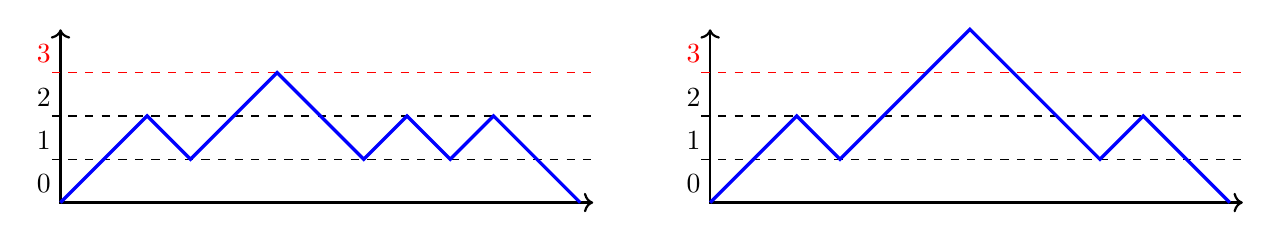
\begin{tikzpicture}[scale=.55]
        \draw[<->, thick] (0, 4) -- (0, 0)  -- (12.3, 0);
        \draw[dashed] (-.2, 1) -- (12.3, 1);
        \draw[dashed] (-.2, 2) -- (12.3, 2);
        \draw[dashed, red] (-.2, 3) -- (12.3, 3);
        \draw[blue, very thick] (0, 0) -- (2, 2) -- (3, 1) -- (5, 3) -- (7, 1) -- (8, 2) -- (9, 1) -- (10, 2) -- (12, 0);
        \draw (0, 0) node[above left] {0};
        \draw (0, 1) node[above left] {1};
        \draw (0, 2) node[above left] {2};
        \draw[red] (0, 3) node[above left] {3};

        \draw[<->, thick] (15+0, 4) -- (15+0, 0)  -- (15+12.3, 0);
        \draw[dashed] (15+-.2, 1) -- (15+12.3, 1);
        \draw[dashed] (15+-.2, 2) -- (15+12.3, 2);
        \draw[dashed, red] (15+-.2, 3) -- (15+12.3, 3);
        \draw[blue, very thick] (15+0, 0) -- (15+2, 2) -- (15+3, 1) -- (15+6, 4) -- (15+9, 1) -- (15+10, 2) -- (15+12, 0);
        \draw (15+0, 0) node[above left] {0};
        \draw (15+0, 1) node[above left] {1};
        \draw (15+0, 2) node[above left] {2};
        \draw[red] (15+0, 3) node[above left] {3};
    \end{tikzpicture}
    \caption{\textbf{On the left}, a valid Dyck word of height 3. \textbf{On the right}, an invalid Dyck word of height 3.}
    \label{fig:dyck_word}
\end{figure}

\subsection{State of the art}
This state of the art will not be to precise as the understanding of the
bibliography has taken almost the first half the internship and will be
more detailed in the \autoref{sec:preli}. First, few years ago Aaronson,
Grier and Schaeffer \cite[2019]{trichotomy_not_andris} worked on quantum complexity
of recognizing regular languages as they can model a lot of tasks. They
concluded that there are 3 different cases depending of the language:
\begin{itemize}
    \item $O(1)$ if it is sufficient to read constant number of letters at the beginning and the end.
    \item $\tilde{\Theta}(\sqrt{n})$ if a Grover's search is the best way to recognize the language.
    \item $\Theta(n)$ if recognizing the language is the same as counting modulo some value that can
          be computed with $O(n)$.
\end{itemize}
Further more, it is proved that being in the second classes is equivalent to
being a star free language. Andris ambainis' team decided to work on \Dyck{k, n} as this
language is a beautiful example of star free languages. In \cite[2020]{art:2DGrid},
the team focus on the power of the logarithm in $\tilde{\Theta}\left(\sqrt{n}\right)$.
They first proved by reduction that the quantum query complexity of \Dyck{k, n}
called $Q\left(\Dyck{k, n}\right)$ is in $\Omega\left(c^k\sqrt{n}\right)$ where $c$ is
a constant greater than 1 and after gave an algorithm for \Dyck{k, n} with a quantum
query complexity of $O\left(\sqrt{n}(\log(n))^{0.5k}\right)$. Since then, no better
lower bound or algorithm have been found.

\subsection{Goals of the internship}
The problem on the quantum query complexity of \Dyck{k,n} is still open, my internship
has for goal to reduce the gap between the lower bound and the best known algorithm.
The researches have been organized on two main axes:
\begin{itemize}
    \item \textbf{Increasing the lower bound.} To do this, It is necessary to understand the bibliography
          on the adversary method in order to try to find a new adversary with better property.
    \item \textbf{Lowering the upper bound.} It is sufficient to find new algorithms
          with a quantum query complexity better than  the previous best known algorithm's one.
\end{itemize}
Finally, the overall goal would be to made the two bounds match in order to get the exact quantum
query complexity of \Dyck{k,n}. Finally, the problem could also be reformulated for multi-brackets word
as done by Kamil Khadiev in \cite{DBLP:conf/uc/KhadievK21}.

\subsection{Results}

{\color{red} \Huge TODO}

\section{Preliminaries}\label{sec:preli}

{ \color{red} Do another plan, to understand this i need to understand this}

\subsection{Quantum query for regular languages.}

In the article \cite{trichotomy_not_andris}, Aaronson, Grier and Schaeffer presented
a really interesting algebraic characterization of regular languages based on the
recognition by monoids and the syntactic congruence. This totally new to me definition
give me some hard time in order to understand it correctly.

\subsection{Regular languages}

Usually, the set of regular languages $\mathcal{R}$ on the alphabet $\Sigma$ is defined as the smallest
fixed point of the function F (the function that computes concatenations, unions, and Kleene stars)
including $\{\varnothing\} \cup \{\varepsilon\} \cup(\cup_{l\in\Sigma}\{l\})$
with F equal:
\begin{align*}\label{eq:F}
    F(X) = & \{AB\  \forall (A,B)\in X^2\}            \\
           & \cup \{A\cup B\ \forall (A,B) \in X^2 \} \\
           & \cup \{A^*\ \forall A \in X \}
\end{align*}
But here, the more convenient way to characterize regular language is with their
algebraic characterization. Indeed, a regular language is always a pre image of a subset
of a monoid under monoid homomorphism. A monoid is a 3-tuple of a set M, an
internal associative binary operation and finally the identity element associated to the
operation. A monoid homomorphism is a map from a monoid to another that preserve the
operation and the identity. The previous property comes from the



\subsubsection{Star free languages}\label{ssec:starfree}

\subsubsection{Trichotomy theorem}



\subsection{The bounds for \Dyck{k,n} problem}

\subsubsection{Lower bound on the quantum query complexity of \Dyck{k, n}}

Explaination of reduction

explaination of adversary methods


\subsubsection{Best known algorithm to recognize \Dyck{k, n}}

Explanation of the algorithm.

\section{A better algorithm for \Dyck{k,n}}

\subsection{A better Complexity Analysis of the original algorithm}

In the article \cite{art:2DGrid}, Andris Ambainis give us a quantum algorithm to recognize
the belonging of a $n$ length bit string in $\Dyck{k, n}$ using
$O(\sqrt{n}(\log_2(n))^{0.5k})$ quantum queries. But the quantum query complexity for $k=1$ is not as good as a
Grover's search which is sufficient. More precisely, for $k=1$ the algorithm is
searching for a minimal $\pm 2$ string in $1x0$ but every minimal $\pm 2$ string
is of size $2$. So the logarithmic search of the upper bound on the size of the
minimal $\pm 2$ string is no more useful and the algorithm can be summarized to
applying a Grover search for 2 consecutive 0 or two consecutive 1. This lower the quantum
query complexity of the initial case of the function to $O(\sqrt{n})$ instead of $O(\sqrt{n\log_2(n)})$.
This give us this following algorithm for \FA{k}.

\begin{algorithm}
    \caption{\FA{k}(l,r,s)}\label{alg:FA_prim}
    \begin{algorithmic}
        \Require $0 \leq l < r$ and $s \subseteq \{1,-1\}$
        \If{$k > 2$}
        \State \textbf{Find} $d$ in $\{2^{\lceil \log_2(k)\rceil }, 2^{\lceil \log_2(k)+1\rceil },\ldots,2^{\lceil \log_2(r-l)\rceil }\}$
        such that \\
        \hspace*{1cm} $v_d \gets $ \FFL{k}$(l,r,d,s)$ is \textbf{not} \Null
        \State \textbf{return} $v_d$ or \Null \ if none
        \Else
        \State \textbf{Find} $t$ in $\{l, l+1, \dots, r\}$ such that \\
        \hspace*{1cm} $v_t \gets$ \FALM{2}$(l,r,t,2,s)$ is \textbf{not} \Null
        \State \textbf{return} $v_t$ of \Null \ if none
        \EndIf
    \end{algorithmic}
\end{algorithm}

The same improvement can be done on \FFP{k} because if $k = 2$ the logarithmic
search is useless. So \FFP{k} can be redefined as in \textsc{Algorithm} \autoref{alg:ffp_better}.
For $k=2$, the complexity is lowered from $O(\sqrt{\log_2(l-r)})$ to $O(1)$.

\begin{algorithm}
    \caption{$\FFP{k}(l,r,t,s)$}\label{alg:ffp_better}
    \begin{algorithmic}
        \Require $0\leq l<r$, $l \leq t \leq r$ and $s \subseteq \{1, -1\}$
        \If{$k>2$}
        \State \textbf{Find} $d$ in $\{2^{\lceil \log_2(k)\rceil }, 2^{\lceil \log_2(k)+1\rceil },\ldots,2^{\lceil \log_2(r-l)\rceil }\}$
        such that \\
        \hspace*{1cm} $v_d \gets $ \FALM{k}$(l,r,t,d,s)$ is \textbf{not} \Null
        \State \textbf{return} $v_d$ or \Null \ if none
        \Else
        \ $v \gets $ \FALM{k}$(l,r,t,2,s)$ is \textbf{not} \Null
        \State \textbf{return} $v_d$ or \Null \ if none
        \EndIf
    \end{algorithmic}
\end{algorithm}

This small improvements on the initial cases will improve the global
quantum query complexity of each subroutine and finally the quantum
query complexity for \Dyck{k,n}.

\newpage

\begin{theorem}{\textbf{\Dyck{k,n}'s algorithm correctness}} \label{th:subroutine_correctness}
    The new definition of \FA{} and \FFP{} does not change the behavior the original algorithm
    as other subroutines (\autoref{annex:complete_subroutine_dyck_kn}) stay unchanged.
\end{theorem}

\begin{tproof}
    The behavior of the \Dyck{k,n} algorithm with the new subroutines is the same than the older
    one as \FA{} (resp. \FF{}) has the same sub-behavior on every entry with its
    older definition.
\end{tproof}

\begin{theorem}{\textbf{\Dyck{k,n}'s Subroutines complexity}} \label{th:subroutine_complexity}
    The subroutines' quantum query complexity for $k$ are the following.
    \begin{enumerate}
        \item $Q$(\Dyck{k,n}) = $O\left(\sqrt{n}(\log_2(n))^{0.5(k-1)}\right)$ \ for $k \geq 1$
        \item $Q$(\FA{k+1}$(l,r,s)$) = $O\left(\sqrt{r-l}(\log_2(r-l))^{0.5(k-1)}\right)$ \ for $k \geq 1$
        \item $Q$(\FFL{k+1}$(l,r,d,s)$) = $O\left(\sqrt{r-l}(\log_2(r-l))^{0.5(k-2)}\right)$ \ for $k \geq 2$
        \item $Q$(\FALM{k+1}$(l, r, t, d, s)$) = $\left\{
                  \begin{array}{ll}
                      O\left(\sqrt{d}(\log_2(d))^{0.5(k-2)}\right) & \textrm{for} \ k \geq 2 \\
                      O(1)                                         & \textrm{for} \  k = 1
                  \end{array}
                  \right.$
        \item $Q$(\FF{k}$(l,r,s, left)$) = $O\left(\sqrt{r-l}(\log_2(r-l))^{0.5(k-2)}\right)$ \ for $k \geq 2$
        \item $Q$(\FFP{k}$(l,r,t,s)$) = $\left\{ \begin{array}{ll}
                      O\left(\sqrt{r-l}(\log_2(r-l))^{0.5(k-2)}\right) & \textrm{for} \ k \geq 3 \\
                      O(1)                                             & \textrm{for} \ k = 2
                  \end{array}
                  \right.$
    \end{enumerate}
\end{theorem}

\begin{tproof}
    The idea is that only the $O\left(\sqrt{n}\right)$ comes from the initial cases for $k = 1$ and
    for each of the $k-1$ level of the recursion, the quantum query complexity is increased by
    a $O\left(\sqrt{\log_2(n)}\right)$ factor. The $O\left(\sqrt{\log_2(n)}\right)$ factor
    is proven by Andris Ambainis' team in \cite{art:2DGrid} while the $O\left(\sqrt{n}\right)$
    for $k = 1$ comes from the new version of \FA{k} (\textsc{Algorithm} \autoref{alg:ffp_better}).
    The complete proof for the theorem is given in \autoref{proof:complexity_dyckkn}.
\end{tproof}

Unfortunately, the improvements done on the initial cases of some of the subroutines are not sufficient
to get a significant improvement for the quantum query complexity of \Dyck{k,n} algorithm. In order to
improve more the query complexity, an other algorithm using a different strategy should be found.

\subsection{A new algorithm for \Dyck{2,n}}

First, we would like to find an algorithm with a quantum query complexity near to match the lower bound,
$\exists c > 1$ such that $Q\left(\Dyck{k,n}\right)=\Omega\left(\sqrt{n}c^k\right)$, describes by Andris
Ambainis' team in \cite{art:2DGrid}. So the searched algorithm must have a quantum query
complexity of $O\left(\sqrt{n}\right)$.

For $k=1$, the query complexity comes only from a call to Grover's search
because rejecting is easily by finding a 00 or a 11 substrings inside the entry. For $k=2$
it no more possible as the substrings that reject are of the form 00(10)*0 or of the form 11(01)*1. It
implies that the number of calls to Grover's search in the naive approach is in $O\left(n\right)$ so the
quantum query complexity finally becomes $O\left(n\sqrt{n}\right)$. In order to keep it in
$O\left(\sqrt{n}\right)$, the algorithm must do a constant number of calls to Grover's search.

For that, we define a new alphabet that can express every even length binary
strings and that have convenient property for a Grover's search. Let
$\mathcal{A} = \{a, b, c, d\}$ the alphabet where $a$ corresponds to 00, $b$ to 11, $c$
to 01, and $d$ to 10. So every string of size 2 has its letter in $\mathcal{A}$ thus every
even length bit string is expressed in $\mathcal{A}^*$. This alphabet allow us to prove the
following theorem.

\begin{theorem}{\textbf{Substrings rejection for Dyck word of height at most 2.}}
    A word on the alphabet $\mathcal{A}$ embodies a Dyck word of
    height at most 2 if and only if it does not contain $aa, ac, bb, bd, cb, cd, da, \textrm{or}\ dc$
    as substrings.
\end{theorem}

\begin{tproof}
    First, this alphabet $\mathcal{A}$ is important because each letter has a height variation
    in $\{-2, 0, 2\}$. Indeed, $a$ has a 2 height variation, $b$ a $-2$, $c$ a 0, and $d$ a 0.
    This means that after each letter in a word, the current height will be even. Moreover,
    for a valid Dyck word of height at most 2, after every letter the height will be 0 or 2
    which are respectively the lower and upper bound for the height. It means that no letter
    can cross a border after its first bit.

    \begin{figure}[h!]
        \centering
        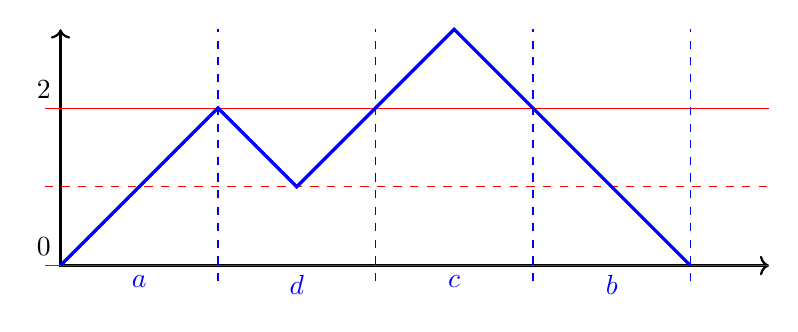
\begin{tikzpicture}
            \draw[<->, thick] (0, 3) -- (0, 0) -- (9, 0);
            \draw[dashed, red] (-.2, 1) --(9, 1);
            \draw[red] (-.2, 2) --(9, 2);
            \draw[red] (-.2, 0) --(9, 0);
            \draw[very thick, blue] (0, 0) -- (2, 2) -- (3, 1) -- (5, 3) -- (8, 0);
            \draw[blue, dashed] (2, -.2) -- (2, 3);
            \draw[blue, dashed] (4, -.2) -- (4, 3);
            \draw[blue, dashed] (6, -.2) -- (6, 3);
            \draw[blue, dashed] (8, -.2) -- (8, 3);
            \draw[blue] (1, 0) node[below] {$a$};
            \draw[blue] (3, 0) node[below] {$d$};
            \draw[blue] (5, 0) node[below] {$c$};
            \draw[blue] (7, 0) node[below] {$b$};
            \draw (0, 2) node[above left] {2};
            \draw (0, 0) node[above left] {0};
        \end{tikzpicture}
        \caption{Illustration of the letters of $\mathcal{A}$ using Dyck's representation.}
        \label{tikz:dyck2alphabet}
    \end{figure}

    This property is important as it implies that every $\pm 3$ strings uses at least two letters.
    So by checking if a pair of letter as a substring of a word make it not a Dyck word, $\mathcal{A}^2$
    can be split into two sets described in \autoref{tab:partitionDyck2}.

    \begin{table}[htb]
        \centering
        \caption{Partition of $\mathcal{A}$ into $\mathcal{X}, \mathcal{V}$.}
        \label{tab:partitionDyck2}
        \begin{tabular}{|c|c|}
            \hline
            $\mathcal{X}$ & $aa$ $ac$ $bb$ $bd$ $cb$ $cd$ $da$ $dc$ \\
            \hline
            $\mathcal{V}$ & $ab$ $ad$ $ba$ $bc$ $ca$ $cc$ $db$ $dd$ \\
            \hline
        \end{tabular}


        \newpage
    \end{table}
    \begin{itemize}
        \item The set $\mathcal{X}$. First, every couple of letter which contains
              a $\pm 3$ strings is in $\mathcal{X}$. This first condition explains the belonging
              of $aa, ac, dc, da, cb, bb, bd, \textrm{and}\ cd $. Next, $cd$ and $dc$ belong
              to $\mathcal{X}$ because of the following property: For any valid Dyck word of
              height at most 2, the current height is bounded between 0 and 2, moreover after each
              letter the current height is even so both couple $cd$ and $dc$ start
              and finish on the same bound. Futhermore,  $cd$ and $dc$ are going
              above and below the height at which they start so both are going outside off the
              bounds, thus a word which contains $cd$ or $dc$ can not be a Dyck Word of height a most 2.
              The \autoref{fig:rejectDyck2} shows each couple of $\mathcal{X}$.

              \begin{figure}[h!]
                  \centering
                  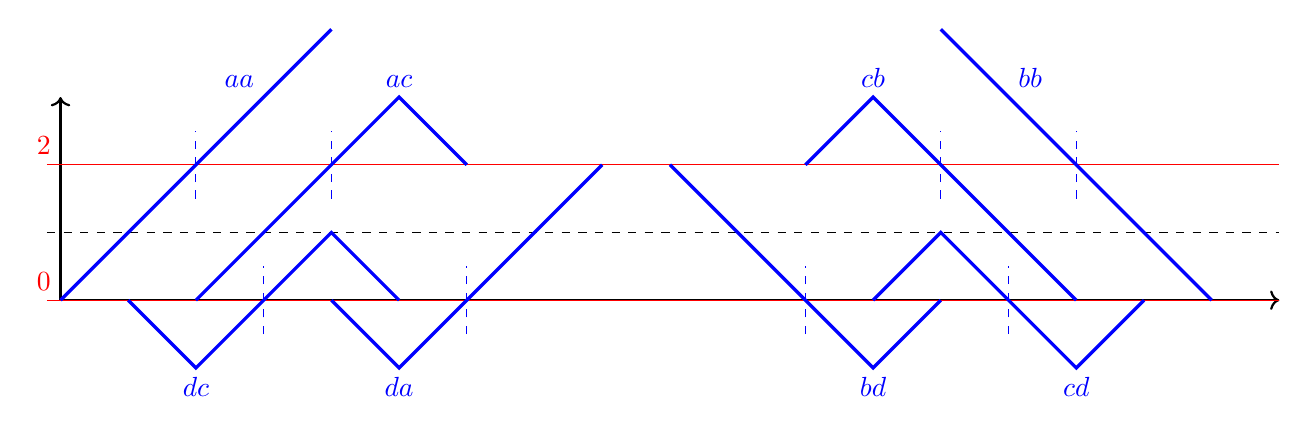
\begin{tikzpicture}[scale=.86]
                      \draw[<->, thick] (0, 3) -- (0, 0) -- (18, 0);
                      \draw[dashed] (-.2, 1) --(18, 1);
                      \draw[red] (-.2, 2) --(18, 2);
                      \draw[red] (-.2, 0) --(18, 0);
                      \draw[blue, very thick] (0, 0) -- (4, 4);
                      \draw[blue, very thick] (1, 0) -- (2, -1) -- (4, 1) -- (5, 0);
                      \draw[blue, very thick] (2,0) -- (5, 3) -- (6, 2);
                      \draw[blue, very thick] (4, 0) -- (5, -1) -- (8, 2);
                      \draw[blue, very thick] (9, 2) -- (12, -1) -- (13, 0);
                      \draw[blue, very thick] (12, 0) -- (13, 1) -- (15, -1) -- (16, 0);
                      \draw[blue, very thick] (11, 2) -- (12, 3) -- (15, 0);
                      \draw[blue, very thick] (13, 4)--(17,0);
                      \draw[red] (0, 2) node[above left] {2};
                      \draw[red] (0, 0) node[above left] {0};
                      \draw[blue] (2, -1) node[below] {$dc$};
                      \draw[blue] (5, -1) node[below] {$da$};
                      \draw[blue] (12, -1) node[below] {$bd$};
                      \draw[blue] (15, -1) node[below] {$cd$};
                      \draw[blue] (3, 3) node[above left] {$aa$};
                      \draw[blue] (5, 3) node[above] {$ac$};
                      \draw[blue] (12, 3) node[above] {$cb$};
                      \draw[blue] (14, 3) node[above right] {$bb$};
                      \draw[blue, dashed] (2, 2-.5) -- (2, 2.5);
                      \draw[blue, dashed] (3, -.5) -- (3, .5);
                      \draw[blue, dashed] (6, -.5) -- (6, .5);
                      \draw[blue, dashed] (4, 2-.5) -- (4, 2.5);
                      \draw[blue, dashed] (3, -.5) -- (3, .5);
                      \draw[blue, dashed] (11, -.5) -- (11, .5);
                      \draw[blue, dashed] (13, 2-.5) -- (13, 2.5);
                      \draw[blue, dashed] (14, -.5) -- (14, .5);
                      \draw[blue, dashed] (15, 1.5) -- (15, 2.5);
                  \end{tikzpicture}
                  \caption{Every 2 letters configuration that implies the word, whom
                      the configuration is a substring, is not a Dyck word of height at most 2.}
                  \label{fig:rejectDyck2}
              \end{figure}

        \item The set $\mathcal{V}$. The couples of $\mathcal{A}$ do not imply
              that the word is not a Dyck word of height at most 2 because each couple
              can fit inside the height bounds. The \autoref{fig:donotrejectDyck2} shows that
              every couple not in $\mathcal{X}$ (ie. $ab, ad, ba, bc, ca, cc, db, dd$)
              fit between height 0 and 2.



              \begin{figure}[h!]
                  \centering
                  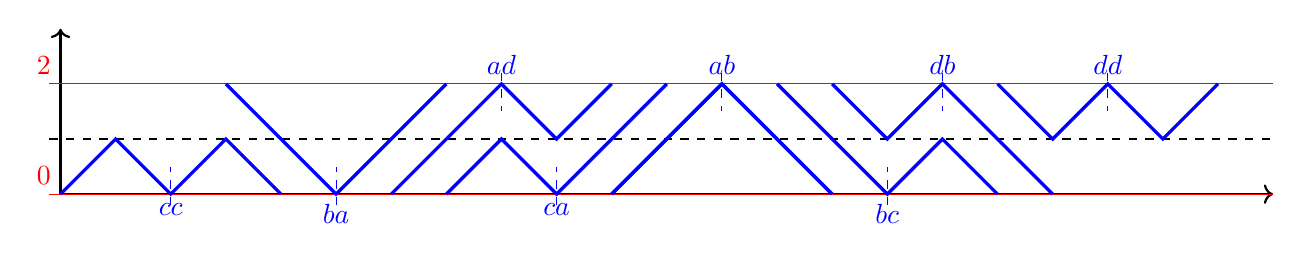
\begin{tikzpicture}[scale=.7]
                      \draw[<->, thick] (0, 3) -- (0, 0) -- (22, 0);
                      \draw[dashed] (-.2, 1) --(22, 1);
                      \draw[red] (-.2, 2) --(22, 2);
                      \draw[red] (-.2, 0) --(22, 0);
                      \draw[red] (0, 2) node[above left] {2};
                      \draw[red] (0, 0) node[above left] {0};
                      \draw[blue, very thick] (10, 0) -- (12, 2) -- (14, 0);
                      \draw[blue, very thick] (13, 2) -- (15, 0) -- (16, 1) -- (17, 0);
                      \draw[blue, very thick] (14, 2) -- (15, 1) -- (16, 2) -- (18, 0);
                      \draw[very thick, blue] (17 ,2) -- (18, 1) -- (19, 2) -- (20, 1) -- (21, 2);
                      \draw[blue, very thick] (10, 0) -- (12, 2) -- (14, 0);
                      \draw[blue, very thick] (11, 2) -- (9, 0) -- (8, 1) -- (7, 0);
                      \draw[blue, very thick] (10, 2) -- (9, 1) -- (8, 2) -- (6, 0);
                      \draw[blue, very thick] (7, 2) -- (5, 0) -- (3, 2);
                      \draw[very thick, blue] (4 ,0) -- (3, 1) -- (2, 0) -- (1, 1) -- (0, 0);
                      \draw[blue] (2, 0) node[below] {$cc$};
                      \draw[blue] (5, 0) node[below] {$ba$};
                      \draw[blue] (8, 2) node[above] {$ad$};
                      \draw[blue] (9, 0) node[below] {$ca$};
                      \draw[blue] (12, 2) node[above] {$ab$};
                      \draw[blue] (15, 0) node[below] {$bc$};
                      \draw[blue] (16, 2) node[above] {$db$};
                      \draw[blue] (19, 2) node[above] {$dd$};
                      \draw[blue, dashed] (2,-.2) -- (2, .5);
                      \draw[blue, dashed] (5, -.2) -- (5, .5);
                      \draw[blue, dashed] (9, -.2) -- (9, .5);
                      \draw[blue, dashed] (8, 2.2) -- (8, 1.5);
                      \draw[blue, dashed] (12, 2.2) -- (12, 1.5);
                      \draw[blue, dashed] (16, 2.2) -- (16, 1.5);
                      \draw[blue, dashed] (19, 2.2) -- (19, 1.5);
                      \draw[blue, dashed] (15, -.2) -- (15, .5);
                  \end{tikzpicture}
                  \caption{Every 2 letters configuration that
                      can be found in a valid Dyck word of height at most 2.}
                  \label{fig:donotrejectDyck2}
              \end{figure}
    \end{itemize}

    So a word, whose letter representation has a substring in $\mathcal{X}$,
    cannot be a Dyck word of height two. But does every non Dyck word of height
    at most 2 have a substring in $\mathcal{X}$?

    A word is not a dyck word of height at most 2 if it include a $\pm 3$ strings.
    But how are represented $\pm 3$ strings using the letters? There are 8
    different cases which are 2 by 2 symmetrical so \autoref{fig:p3string}
    and \autoref{fig:p3string2piece} show only the cases for +3 strings. In
    \autoref{fig:p3string}, every +3 string of size 3 is include in $aa$ or
    $ac$ so it is sufficient to search for this two couple. In \autoref{fig:p3string2piece}
    every +3 strings of length greater than 3 are composed of 2 minimal +2
    strings. This implies that one must be a $a$ while the other must be $da$
    of $dc$. Because $da$ or $dc$ are rejecting substrings, it is sufficient
    to search for them.

    \begin{figure}[h!]
        \begin{minipage}{.35\textwidth}
            \centering
            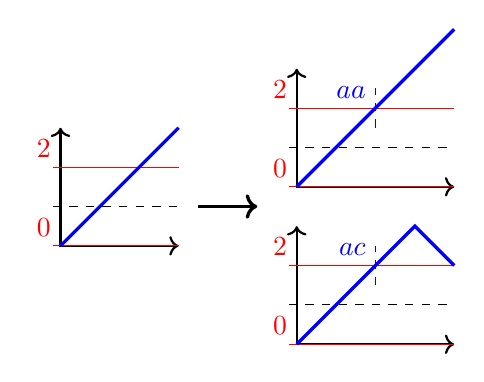
\begin{tikzpicture}[scale=.5]
                \draw[<->, thick] (0, 3) -- (0, 0) -- (3, 0);
                \draw[dashed] (-.2, 1) --(3, 1);
                \draw[red] (-.2, 2) --(3, 2);
                \draw[red] (-.2, 0) --(3, 0);
                \draw[red] (0, 2) node[above left] {2};
                \draw[red] (0, 0) node[above left] {0};
                \draw[blue, very thick] (0, 0) -- (3, 3);
                \draw[->, very thick] (3.5, 1) -- (5, 1);

                \draw[<->, thick] (6, 4+.5) -- (6, 1+.5) -- (10, 1+.5);
                \draw[dashed] (5.8,2+.5) -- (10,2+.5);
                \draw[red] (5.8,3+.5) -- (10,3+.5);
                \draw[red] (5.8,1+.5) -- (10, 1+.5);
                \draw[red] (6, 3+.5) node[above left] {2};
                \draw[red] (6, 1+.5) node[above left] {0};
                \draw[blue, very thick] (6, 1+.5) -- (10, 5+.5);
                \draw[blue, dashed] (8, 2.5+.5) -- (8, 3.5+.5);
                \draw[blue] (8, 3+.5) node[above left] {$aa$};

                \draw[<->, thick] (6, 4-4+.5) -- (6, 1-4+.5) -- (10, 1-4+.5);
                \draw[dashed] (5.8,2-4+.5) -- (10,2-4+.5);
                \draw[red] (5.8,3-4+.5) -- (10,3-4+.5);
                \draw[red] (5.8,1-4+.5) -- (10, 1-4+.5);
                \draw[red] (6, 3-4+.5) node[above left] {2};
                \draw[red] (6, 1-4+.5) node[above left] {0};
                \draw[blue, very thick] (6, 1-4+.5) -- (9, 0+.5) -- (10, -1+.5);
                \draw[blue, dashed] (8, 2.5-4+.5) -- (8, 3.5-4+.5);
                \draw[blue] (8, 3-4+.5) node[above left] {$ac$};
            \end{tikzpicture}
            \caption{Configuration for a +3 strings of size 3.}
            \label{fig:p3string}
        \end{minipage}
        \hfill
        \begin{minipage}{.60\textwidth}
            \centering
            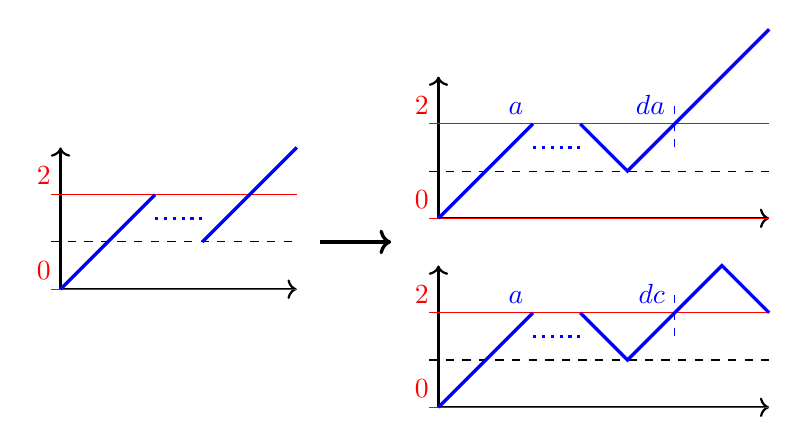
\begin{tikzpicture}[scale=.6]
                \draw[<->, thick] (0, 3) -- (0, 0) -- (5, 0);
                \draw[dashed] (-.2, 1) --(5, 1);
                \draw[red] (-.2, 2) --(5, 2);
                \draw[red] (-.2, 0) --(5, 0);
                \draw[red] (0, 2) node[above left] {2};
                \draw[red] (0, 0) node[above left] {0};
                \draw[blue, very thick] (0, 0) -- (2, 2);
                \draw[blue, very thick, dotted] (2, 1.5) -- (3, 1.5);
                \draw[blue, very thick] (3, 1) -- (5, 3);
                \draw[->, very thick] (5.5, 1) -- (7, 1);

                \draw[<->, thick] (8+0, 3+1.5) -- (8+0, 0+1.5) -- (8+5+2, 0+1.5);
                \draw[dashed] (8+-.2, 1+1.5) --(8+5+2, 1+1.5);
                \draw[red] (8+-.2, 2+1.5) --(8+5+2, 2+1.5);
                \draw[red] (8+-.2, 0+1.5) --(8+5+2, 0+1.5);
                \draw[red] (8+0, 2+1.5) node[above left] {2};
                \draw[red] (8+0, 0+1.5) node[above left] {0};
                \draw[blue, very thick] (8+0, 0+1.5) -- (8+2, 2+1.5);
                \draw[blue, very thick, dotted] (8+2, 1.5+1.5) -- (8+3, 1.5+1.5);
                \draw[blue, very thick] (8+3, 2+1.5) -- (8+4, 1+1.5) -- (8+7, 4+1.5);
                \draw[blue, dashed] (13, 1.5+1.5) -- (13, 4);
                \draw[blue] (13, -.5+4) node[above left] {$da$};
                \draw[blue] (10, -.5+4) node[above left] {$a$};

                \draw[<->, thick] (8+0, 3+1.5-4) -- (8+0, 0+1.5-4) -- (8+5+2, 0+1.5-4);
                \draw[dashed] (8+-.2, 1+1.5-4) --(8+5+2, 1+1.5-4);
                \draw[red] (8+-.2, 2+1.5-4) --(8+5+2, 2+1.5-4);
                \draw[red] (8+-.2, 0+1.5-4) --(8+5+2, 0+1.5-4);
                \draw[red] (8+0, 2+1.5-4) node[above left] {2};
                \draw[red] (8+0, 0+1.5-4) node[above left] {0};
                \draw[blue, very thick] (8+0, 0+1.5-4) -- (8+2, 2+1.5-4);
                \draw[blue, very thick, dotted] (8+2, 1.5+1.5-4) -- (8+3, 1.5+1.5-4);
                \draw[blue, very thick] (8+3, 2+1.5-4) -- (8+4, 1+1.5-4) -- (8+6, 3+1.5-4) -- (8+7, 2+1.5-4);
                \draw[blue, dashed] (13, -1) -- (13, 0);
                \draw[blue] (13, -.5) node[above left] {$dc$};
                \draw[blue] (10, -.5) node[above left] {$a$};

            \end{tikzpicture}
            \caption{Configurations for a +3 string of size greater than 3.}
            \label{fig:p3string2piece}
        \end{minipage}
    \end{figure}

\end{tproof}
Finally, a word on the alphabet $\mathcal{A}$ embodies a Dyck word of
height at most 2 if and only if it does not contain $aa, ac, bb, bd, cb, cd, da, dc$
as substrings. The following \textsc{Algorithm} \autoref{alg:dyck2nsqrt} for \Dyck{2, n}
comes from the direct application of the theorem.


\begin{algorithm}
    \caption{\textsc{DyckFast}$_{2,n}$}\label{alg:dyck2nsqrt}
    \begin{algorithmic}
        \Require $n \geq 0$, $x$ such that  $|x| = 2n$
        \State $x \gets 11x00$
        \State $\texttt{t} \gets \Null$
        \For{$\texttt{reject\_symbol} \in \{aa, ac, bb, bd, cb, cd, da, dc\}$}
        \If{$t == \Null$}
        \State \textbf{Find} $\texttt{t}$ in $\llbracket0, n\rrbracket$ such that \\
        \hspace*{1cm} $x[2\texttt{t}, \ldots, 2\texttt{t}+3] = \texttt{reject\_symbol}$
        \EndIf
        \EndFor
        \State \textbf{return} $\texttt{t} == \Null$

    \end{algorithmic}
\end{algorithm}

\begin{theorem}{\textbf{The quantum query complexity of \textsc{DyckFast}$_{2,n}$.}}
    The \textsc{DyckFast}$_{2,n}$ algorithm has a quantum query complexity of $O\left(\sqrt{n}\right)$.
\end{theorem}

\begin{tproof}
    The algorithm is doing at most 8 Grover's search on the modified input string $11x00$.
    So the total quantum query complexity is the folling.
    \[Q(\textsc{DyckFast}_{2, n}) = 8\times O\left(\sqrt{n+4}\right) = O\left(\sqrt{n}\right)\]
\end{tproof}

\subsection{A new algorithm for k=3}

\subsection{A try for a new algorithm for any k.}



\section{Conclusion}

Conclusion here.


\bibliographystyle{plain}
\bibliography{biblio}
\listoffigures
\listofalgorithms

\newpage

\section{Appendix}

\begin{appendix}

    \section*{The frame of the intership}

    \section{The algorithm for \Dyck{k, n}}
    \label{annex:complete_subroutine_dyck_kn}
    All the subroutines' pseudo code can be found from \textsc{Algorithm}
    \autoref{alg:dyck_kn} to \textsc{Algorithm} \autoref{alg:ffp}.

    \begin{algorithm}
        \caption{\Dyck{k,n}}\label{alg:dyck_kn}
        \begin{algorithmic}
            \Require $n \geq 0$ and $k \geq 1$
            \Ensure $|x| = n $
            \State $x \gets 1^kx0^k$
            \State $v \gets$ \FA{k+1}$(0, n+2*k-1, \{1,-1\})$
            \State \textbf{return} v = \Null
        \end{algorithmic}
    \end{algorithm}

    \begin{algorithm}
        \caption{\FA{k}$(l,r,s)$}\label{alg:fa_k}
        \begin{algorithmic}
            \Require $0 \leq l < r$ and $s \subseteq \{1,-1\}$
            \State \textbf{Find} $d$ in $\{2^{\lceil \log_2(k)\rceil }, 2^{\lceil \log_2(k)+1\rceil },\ldots,2^{\lceil \log_2(r-l)\rceil }\}$
            such that \\
            \hspace*{1cm} $v_d \gets $ \FFL{k}$(l,r,d,s)$ is \textbf{not} \Null
            \State \textbf{return} $v_d$ or \Null \ if none
        \end{algorithmic}
    \end{algorithm}

    \begin{algorithm}
        \caption{\FFL{k}$(l,r,d,s)$}\label{alg:ffl_k}
        \begin{algorithmic}
            \Require $0 \leq l < r$, $1\leq d \leq r-l$ and $s \subseteq \{1,-1\}$
            \State \textbf{Find} $t$ in $\{l, l+1, \dots, r\}$ such that \\
            \hspace*{1cm} $v_t \gets$ \FALM{k}$(l,r,t,d,s)$ is \textbf{not} \Null
            \State \textbf{return} $v_t$ of \Null if none
        \end{algorithmic}
    \end{algorithm}

    \begin{algorithm}
        \caption{\FALM{k}$(l,r,d,t,s)$}\label{alg:falm_k}
        \begin{algorithmic}
            \Require $0 \leq l < r$, $l \leq r \leq r$, $1\leq d \leq r-l$ and $s \subseteq \{1,-1\}$
            \State $v = (i_1,j_1,\sigma_1) \gets \FALM{k-1}(l,r,t,d-1,\{1,-1\})$
            \If{$v \neq \Null$} {
                \State $v' = (i_2,j_2,\sigma_2) \gets \FARM{k-1}(l,r,i_1-1,d-1,\{1,-1\})$
                \If{$v' = \Null$}
                \State $v' = (i_2,j_2,\sigma_2) \gets \FF{k-1}(\max(l, j_1-d+1),i_1-1,\{1,-1\}, left)$
                \EndIf
                \If{$v'\neq \Null$ and $\sigma_2 \neq \sigma_1$}{\ $v' \gets \Null$}
                \EndIf
                \If{$v' = \Null$}
                \State $v' = (i_2,j_2,\sigma_2) \gets \FALM{k-1}(l,r,j_1+1,d-1,\{1,-1\})$
                \EndIf
                \If{$v' = \Null$}
                \State $v' = (i_2,j_2,\sigma_2) \gets \FF{k-1}(j_1+1,\max(r, i_1+d-1),\{1,-1\}, right)$
                \EndIf
                \If{$v' = \Null$}{\ \textbf{return} \Null}
                \EndIf
            }
            \Else {
            \State $v = (i_1,j_1,\sigma_1) \gets \FF{k-1}(t, min(t+d-1, r), \{1,-1\}, right)$
            \If{v = \Null}{\ \textbf{return} \Null}
            \EndIf
            \State $v' = (i_2, j_2, \sigma_2) \gets \FF{k-1}(max(t-d+1, l), t, \{1, -1\}, left)$
                \If{$v' = \Null$}{\ \textbf{return} \Null}
                \EndIf
                }
                \EndIf
                \If{$\sigma_1=\sigma_2$ and $\sigma_1 \in s$ and $\max(j_1, j_2) - \min(i_1, i_2) + 1 \leq d$}
                \State \textbf{return} $(\min(i_1, i_2), \max(j_1, j_2), \sigma_1)$
            \Else{\ \textbf{return} \Null}
            \EndIf

        \end{algorithmic}
    \end{algorithm}

    \begin{algorithm}
        \caption{\FF{k}$(l, r, s, left)$}
        \begin{algorithmic}
            \Require $0\leq l < r$ and $s \subseteq \{1,-1\}$
            \State $lBorder \gets l, rBorder \gets r, d \gets 1$
            \While{$lBorder + 1 < rBorder $}
            \State $ mid \gets \lfloor (lBorder + rBorder)/2 \rfloor $
            \State $v_l \gets \FA{k}(lBorder, mid, s)$
            \If{$v_l \neq \Null$}{\ $rBorder \gets mid$}
            \Else
            \State $v_{mid} \gets \FFP{k}(lBorder, rBorder, mid, s, left)$
            \If{$v_{mid} \neq \Null$}{\ \textbf{return} $v_{mid}$}
            \Else{\ $lBorder \gets mid + 1$}
            \EndIf
            \EndIf
            \State $d \gets d+1$
            \EndWhile
            \State \textbf{return} \Null
        \end{algorithmic}
    \end{algorithm}


    \begin{algorithm}
        \caption{$\FFP{k}(l,r,t,s)$}\label{alg:ffp}
        \begin{algorithmic}
            \Require $0\leq l<r$, $l \leq t \leq r$ and $s \subseteq \{1, -1\}$

            \State \textbf{Find} $d$ in $\{2^{\lceil \log_2(k)\rceil }, 2^{\lceil \log_2(k)+1\rceil },\ldots,2^{\lceil \log_2(r-l)\rceil }\}$
            such that \\
            \hspace*{1cm} $v_d \gets $ \FALM{k}$(l,r,t,d,s)$ is \textbf{not} \Null
            \State \textbf{return} $v_d$ or \Null \ if none
        \end{algorithmic}
    \end{algorithm}

    \section{The proof of the quantum query complexity for \Dyck{k,n} algorithm's subroutines}
    \label{proof:complexity_dyckkn}

    \begin{theorem}{\textbf{\Dyck{k,n}'s Subroutines complexity}} \label{th:subroutine_complexity}
        The subroutines' quantum query complexity for $k$ are the following.
        \begin{enumerate}
            \item $Q$(\Dyck{k,n}) = $O\left(\sqrt{n}(\log_2(n))^{0.5(k-1)}\right)$ \ for $k \geq 1$
            \item $Q$(\FA{k+1}$(l,r,s)$) = $O\left(\sqrt{r-l}(\log_2(r-l))^{0.5(k-1)}\right)$ \ for $k \geq 1$
            \item $Q$(\FFL{k+1}$(l,r,d,s)$) = $O\left(\sqrt{r-l}(\log_2(r-l))^{0.5(k-2)}\right)$ \ for $k \geq 2$
            \item $Q$(\FALM{k+1}$(l, r, t, d, s)$) = $\left\{
                      \begin{array}{ll}
                          O\left(\sqrt{d}(\log_2(d))^{0.5(k-2)}\right) & \textrm{for} \ k \geq 2 \\
                          O(1)                                         & \textrm{for} \  k = 1
                      \end{array}
                      \right.$
            \item $Q$(\FF{k}$(l,r,s, left)$) = $O\left(\sqrt{r-l}(\log_2(r-l))^{0.5(k-2)}\right)$ \ for $k \geq 2$
            \item $Q$(\FFP{k}$(l,r,t,s)$) = $\left\{ \begin{array}{ll}
                          O\left(\sqrt{r-l}(\log_2(r-l))^{0.5(k-2)}\right) & \textrm{for} \ k \geq 3 \\
                          O(1)                                             & \textrm{for} \ k = 2
                      \end{array}
                      \right.$
        \end{enumerate}
    \end{theorem}

    \begin{tproof} The proof is done by induction on the height $k$ of the Dyck word.
        \init{For $k=1$ and $k=2$ we have the following initialization. \\
            \begin{itemize}
                \item For $k=1$, only \FALM{2}, \FA{2} ,and \Dyck{1,n} are defined. The $O(1)$ quantum query complexity
                      of \FALM{2} comes directly from the definition of its initial case, as the $O(\sqrt{r-l})$ quantum
                      query complexity of \FA{2}. Then the $O\left(\sqrt{n}\right)$ quantum query complexity of \Dyck{1,n} comes from
                      the call to \FA{2}.
                \item For $k=2$, the inductive part of the algorithm start and every subroutines is defined. The $O(1)$
                      quantum query complexity of \FFP{2} comes from the call to \FALM{2}.
                      The $O\left(\sqrt{r-l}\right)$ quantum query complexity of \FF{2} comes from the dichotomize search using \FA{2} and
                      \FFP{2} because $\sum_{u=1}^{log_2(r-l)}2u\left(O\left(\sqrt{\frac{r-l}{2^{u-1}}}\right)+O(1)\right) = O(\sqrt{r-l})$
                      (Detailed in the induction). The $O(\sqrt{d})$ quantum query complexity of \FALM{3} comes from the
                      constant amount of calls to \FF{2} and \FALM{2} with entry of size $d$. The $O(\sqrt{r-l})$ quantum query
                      complexity of \FFL{3} comes from the $O\left(\sqrt{\frac{r-l}{d}}\right)$ calls to \FALM{3}. The $O\left(\sqrt{(r-l)\log_2(r-l)}\right)$
                      quantum query complexity of \FA{3} comes from the $O\left(\sqrt{\log_2(r-l)}\right)$ calls to \FFL{3}. Finally, the
                      $O\left(\sqrt{(r-l)\log_2(r-l)}\right)$ quantum query complexity of \Dyck{2} comes from the call to \FA{3}.
            \end{itemize}
        }
        \hered{Let suppose it exists $k$ such that \autoref{th:subroutine_complexity} is
            true for $k$. Let prove that it is true for $k+1$. \\

            First, the $O\left(\sqrt{r-l}(\log_2(r-l))^{0.5(k-1)}\right)$ quantum query complexity of \FFP{k+1} comes from
            the $O\left(\sqrt{\log(r-l)}\right)$ calls to \FALM{k+1}.
            \begin{align*}
                Q(\textrm{\FFP{k+1}}(l, r, t, s)) & = O(\sqrt{\log(r-l)}) \times O\left(Q(\textrm{\FALM{k+1}}(l, r, t, d, s))\right)\            \\
                                                  & \overset{IH}{=} O \left( \sqrt{\log(r-l)} \times \sqrt{r-l}(\log_2(r-l))^{0.5(k-2)}  \right) \\
                                                  & = O \left( \sqrt{r-l}(\log_2(r-l))^{0.5(k-1)} \right)
            \end{align*}

            Thus the $O \left(\sqrt{r-l}(\log_2(r-l))^{0.5(k-2)}\right)$ quantum query complexity of \FF{k+1} comes
            from the dichotomize search using calls to \FA{k+1} and \FF{k+1}.

            \blfootnote{\begin{align*}
                    ^{a}\sum_{u=1}^{+\infty} \left(\frac{\textrm{d}}{\textrm{d}x}(x^{u})\right)\left(\frac{1}{\sqrt{2}}\right)
                    \leq \left(\frac{\textrm{d}}{\textrm{d}x} \left( \sum_{u=1}^{+\infty} x^u \right)\right)\left(\frac{1}{\sqrt{2}}\right)
                    \leq \left(\frac{\textrm{d}}{\textrm{d}x} \left( \frac{x}{1-x} \right)\right)\left(\frac{1}{\sqrt{2}}\right)
                    \leq \left(\frac{1}{(1-x)^2}\right)\left(\frac{1}{\sqrt{2}}\right)
                    \leq \frac{1}{(1-\frac{1}{\sqrt{2}})^2} \leq \frac{\sqrt{2}^2}{(\sqrt{2} - 1)^2}
                \end{align*}}

            \begin{align*}
                Q(\textrm{\FF{k+1}}(l,r,t,d,s)) & = \begin{array}{l}
                    \sum_{u=1}^{\log_2(r-l)}2u \times O\left(Q(\textrm{\FA{k+1}}(0, \frac{r-l}{2^{u-1}}, s))\right) \\
                    + \sum_{u=1}^{\log_2(r-l)}2u \times O\left(Q(\textrm{\FFP{k+1}}(0, \frac{r-l}{2^{u-1}}, \_ , s, left))\right)
                \end{array}                                                     \\
                                                & \overset{IH}{=}
                O\left(\sum_{u=1}^{\log_2(r-l)}2u \times \sqrt{\frac{r-l}{2^{u-1}}}(\log_2(\frac{r-l}{2^{u-1}}))^{0.5(k-1)}\right) \\
                                                & =
                O\left(\sum_{u=1}^{\log_2(r-l)}2u \times \sqrt{\frac{r-l}{2^{u-1}}}(\log_2(r-l))^{0.5(k-1)}\right)                 \\
                                                & =
                O \left(\sqrt{r-l}(\log_2(r-l))^{0.5(k-1)}\sum_{u=1}^{\log_2(r-l)}u\times (\frac{1}{\sqrt{2}})^{u-1} \right)       \\
                                                & =^{a}
                O \left(\sqrt{r-l}(\log_2(r-l))^{0.5(k-1)} \frac{\sqrt{2}^2}{(\sqrt{2}-1)^2}\right)                                \\
                                                & =
                O \left(\sqrt{r-l}(\log_2(r-l))^{0.5(k-1)}\right)
            \end{align*}


            Next, the $ O\left(\sqrt{d}(\log_2(d))^{0.5(k-1)} \right)$ quantum query complexity comes of \FALM{k+2}from the constant amount
            of calls to \FALM{k+1}, \FARM{k+1} ,and \FF{k+1}.

            \begin{align*}
                Q(\textrm{\FALM{k+2}}(l,r,t,d,s)) & = \begin{array}{l}
                    3 \times O\left(Q(\textrm{\FALM{k+1}}(l,r,t,d,\{1,-1\}))\right) \\
                    + 4 \times O\left(Q(\textrm{\FF{k+1}}(l,r,\{1,-1\},left))\right)
                \end{array}                                  \\
                                                  & \overset{IH}{=} O\left(\sqrt{d}(\log_2(d))^{0.5(k-1)} \right)
            \end{align*}

            After that, the $O\left( \sqrt{r-l}(\log_2(r-l))^{0.5(k-1)}\right)$ quantum query complexity of \FFL{k+2} comes from the
            $O\left(\sqrt{\frac{r-l}{d}}\right)$ calls to \FALM{k+2}.

            \begin{align*}
                Q(\textrm{\FFL{k+2}}(l, r, d, s)) & = O\left(\sqrt{\frac{r-l}{d}}\right) \times O\left(Q(\textrm{\FALM{k+2}}(l,r,t,d,s))\right) \\
                                                  & = O\left( \sqrt{\frac{r-l}{d}} \times \sqrt{d}(\log_2(d))^{0.5(k-1)}\right)                 \\
                                                  & = O\left( \sqrt{r-l}(\log_2(d))^{0.5(k-1)}\right)                                           \\
                                                  & = O\left( \sqrt{r-l}(\log_2(r-l))^{0.5(k-1)}\right)
            \end{align*}

            Hence the $O\left( \sqrt{r-l}(\log_2(r-l))^{0.5k} \right)$ quantum query complexity of \FA{k+2} comes from the
            the $O\left(\sqrt{\log_2(r-l)}\right)$ calls to \FFL{k+2}.

            \begin{align*}
                Q(\textrm{\FA{k+2}}(l, r, s)) & = O\left(\sqrt{\log(r-l)}\right) \times O\left(Q(\textrm{\FFL{k+2}}(l, r, d, s))\right) \\
                                              & = O\left( \sqrt{\log(r-l)} \times \sqrt{r-l}(\log_2(r-l))^{0.5(k-1)} \right)            \\
                                              & = O\left( \sqrt{r-l}(\log_2(r-l))^{0.5k} \right)                                        \\
            \end{align*}

            Finally, the $O\left( \sqrt{n}(\log_2(n))^{0.5k} \right)$ quantum query complexity of \Dyck{k+1,n} comes from the
            call to \FA{k+2}.

            \begin{align*}
                Q(\textrm{\Dyck{k+1,n}}) & = O\left(Q(\textrm{\FA{k+2}}(0,n+2k+1,s))\right) \\
                                         & = O\left(Q(\textrm{\FA{k+2}}(0, n, s))\right)    \\
                                         & = O\left( \sqrt{n}(\log_2(n))^{0.5k} \right)
            \end{align*}

        }

        \Conc{By the induction principle we get that the \autoref{th:subroutine_complexity} is true for $k \in \mathbb{N}^*$}
    \end{tproof}

\end{appendix}

\end{document}